\section{Derivazione del modello}
Consideriamo una corda di lunghezza $L$ e densit\`a lineare di massa $\rho_0$
costante a riposo.\\
Sia $t≥ 0$ il tempo, $x \in [0,L]$ la posizione in orizzontale,
$u(t,x)$ lo spostamento in verticale dalla posizione di riposo durante la
vibrazione della corda che pensiamo perfettamente flessibile.
Lo spostamento \`e assunto solo verticale e con vibrazioni di piccola ampiezza
rispetto ad L. Si trascurano gli attriti.\\
Si parte dalla conservazione della massa. Indichiamo con $\rho (t,x)$ la
densit\`a
lineare di massa al tempo $t$ nella posizione $x$. L'elemento di lunghezza al
tempo (fissato) $t$ \`e
\[
	ds=\sqrt{1+u_x^2} dx
\]
visto che si ha a che fare con una curva cartesiana
\[
	\left\{
	\begin{array}{ll}
		\begin{array}{l}
			x=x \\
			u=u(t,x)
		\end{array}
	& 0 ≤ x ≤ L
	\end{array}
	\right.
\]
nel piano $x,u$
\begin{figure}[H]
	\centering
	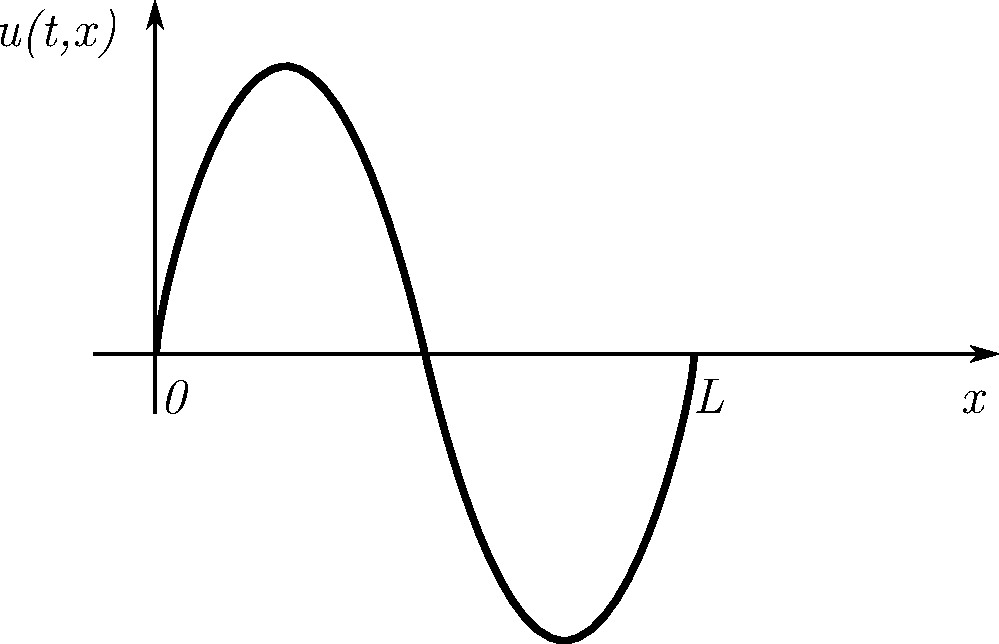
\includegraphics[width=0.6\textwidth]{wave_plane.pdf}
	\caption{$u(t,x)$ con $t$ fissato.}
	\label{wave_plane}
\end{figure}
La conservazione della massa si scrive
\[
	\rho ds= \rho_0 dx
\]
quindi
\[
	\rho \sqrt{1 + u_x^2}= \rho_0
\]
Ora imponiamo che le componenti orizzontali delle forze si bilancino, dato lo
spostamento solo verticale.
Assumiamo che l'unica forza non completamente verticale  applicata nei punti
della corda, sia la tensione, forza diretta tangenzialmente data la corda
perfettamente
flessibile.
Precisamente, il vettore tensione ${\bf T}(t,x)$ indica la forza che la porzione
di corda a distanza dal punto $(x, u(t,x))$ esercita sulla porzione a sinistra.
Evidentemente ${\bf -T}(t,x)$ \`e la forza che la porzione a sinistra esercita
su
quella a destra.
\begin{figure}[H]
	\centering
	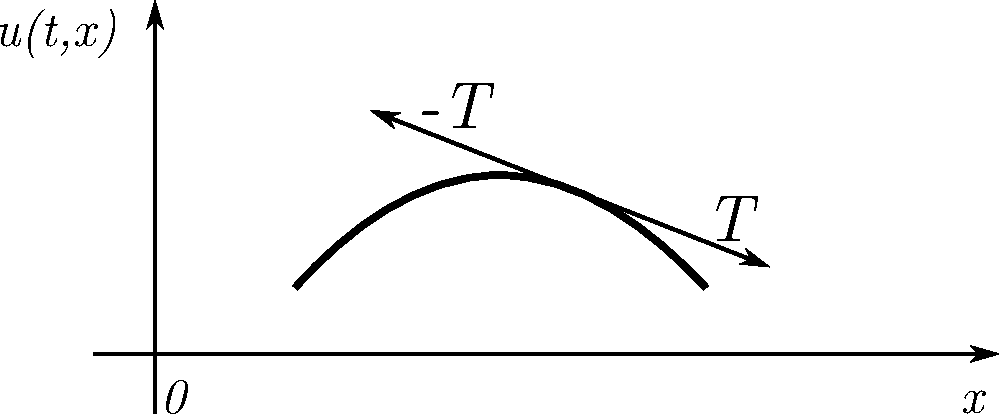
\includegraphics[width=0.6\textwidth]{tension.pdf}
	\caption{Tensione sulla corda.}
	\label{tension}
\end{figure}
Indichiamo con $T(t,x)$ l'intensit\`a di ${\bf T}(t,x)$ e con $\alpha= \alpha
(t,x)$
l'inclinazione della corda rispetto alla posizione di riposo (asse $x$).
\[
	tg \alpha = u_x
\]
\begin{figure}[H]
	\centering
	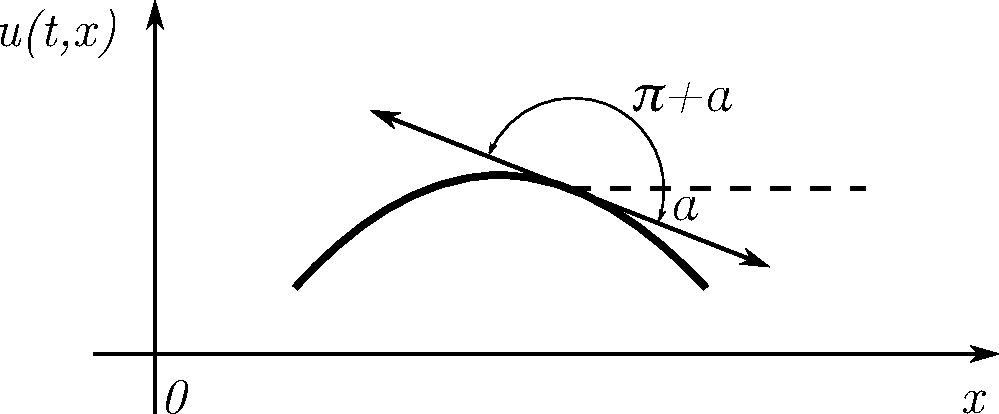
\includegraphics[width=0.6\textwidth]{tension_alpha.pdf}
	\caption{Tensione sulla corda con $\alpha$ mostrato.}
	\label{tension_alpha}
\end{figure}
Il bilancio della componente orizzontale della tensione in un breve intervallo
$[x,x+\Delta x]$ impone
\[
	cos(\alpha + \pi)= - cos \alpha
\]
\begin{figure}[H]
	\centering
	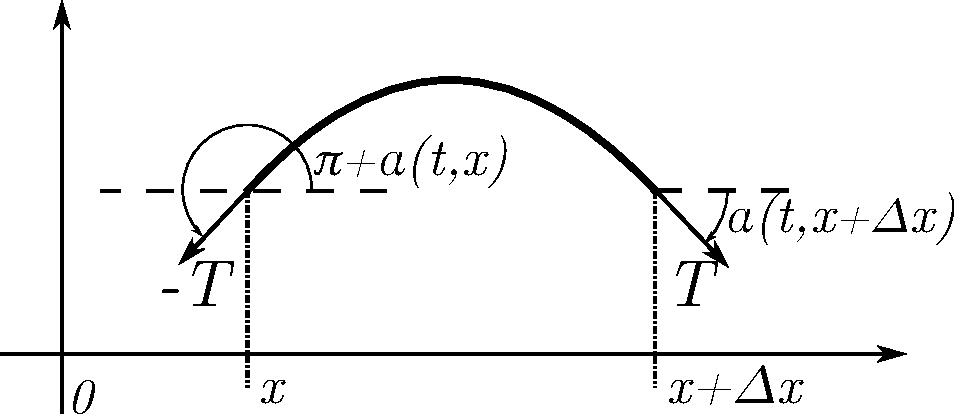
\includegraphics[width=0.8\textwidth]{tension_dx.pdf}
	\caption{Tensione sulla corda tra due punti distanti $dx$.}
	\label{tension_dx}
\end{figure}
\[
	T(t, x + \Delta x) cos \; \alpha(t, x + \Delta x)-
	T(t,x)cos \; \alpha(t,x)=0
\]
Dividendo per $\Delta x$ e mandando $\Delta x \to 0$
\[
	\frac{\partial}{\partial x}[T(t,x) cos \; \alpha(t,x)]=0
\]
da cui
\[
	T(t,x) cos \; \alpha(t,x)= \tau
\]
con $\tau$ indipendente da $x$.
La componente orizzontale della tensione, detta trazione, non dipende dalla
posizione. Se assumiamo che la tensione sia di intensit\`a proporzionale
alla lunghezza della porzione di corda che la esercita, allora $\tau$ \`e
indipendente anche da $t$ visto che la lunghezza in orizzontale \`e costante
$L$.\\
Calcoliamo ora la componente verticale della tensione nel tratto di corda
corrispondente a $[x, x+ \Delta x]$. Tenendo conto di $sin(\alpha + \pi)= - sin
\alpha$ e di $T= \tau/cos\alpha$, essa vale
\[
	T(t,x+\Delta x)sin \, \alpha(t, x+ \Delta x) - T(t,x)sin \, \alpha
(t,x)=
\]
\[
	\tau[tg \, \alpha (t, x + \Delta x)- tg  \, \alpha(t,x)]=
\]
\[
	\tau[u_x \, \alpha (t, x + \Delta x)- u_x \alpha(t,x)]=
	\tau \int_x^{x+\Delta x} u_{xx}(t,y) dy
\]
Essendo una trazione, essa corrisponde ad una forza.\\
Denotiamo ora con $f(t,x)$ gli eventuali carichi totali per unit\`a di massa; se
il
peso non \`e trascurabile $f(t,x)= -g + F(t,x)$ dove $g$ \`e l'accelerazione
di gravit\`a ed $F$ corrisponde ad altri ulteriori carichi. Quindi
\[
	=\tau \int_x^{x+\Delta x} u_{xx}(t,y) dy +
	\int_x^{x+\Delta x} f(t,y) \rho (t,y) \sqrt{1+ u_x^2(t,y)} dy
\]
Per il principio fondamentale della dinamica, forza = massa $\cdot$
accelerazione rappresenta sempre una forza
\[
	\underbrace{\int_x^{x+\Delta x} u_{tt}(t,y) \rho (t,y) \sqrt{1+
u_x^2(t,y)} dy}_{
	\text{accelerazione $\cdot$ massa}}
\]
perci\`o
\begin{align*}
	\int_x^{x+\Delta x} u_{tt}(t,y) \rho (t,y) \sqrt{1+ u_x^2(t,y)} dy&= \\
	\tau \int_x^{x+\Delta x} u_{xx}(t,y) dy &+
	\int_x^{x+\Delta x} f(t,y) \rho (t,y) \sqrt{1+ u_x^2(t,y)} dy
\end{align*}
che pu\`o essere scritta
\[
	\int_x^{x+\Delta x}\rho_0 u_{tt}(t,y)  dy=
	\int_x^{x+\Delta x} \tau u_{xx}(t,y) dy +
	\int_x^{x+\Delta x} \rho_0 f(t,y)  dy
\]
\[
	\int_x^{x+\Delta x} \left[
	\rho_0 u_{tt} - \tau u_{xx}-  \rho_0 f
	\right]dy= 0
\]
Per l'arbitrariet\`a del tratto $[x, x+ \Delta x]$, deve essere
\[
	\rho_0 u_{tt} - \tau u_{xx}-  \rho_0 f
\]
Dividendo per $\rho_0$ ed indicando $c^2=\tau / \rho_0$ si ha l'equazione
\[
	u_{tt} - c^2 u_{xx} = f
\]
La costante $c$ ha la dimensione di una velocit\`a.
\section{Problemi ben posti con lunghezza finita}
Esistenza, unicit\`a e dipendenza continua dai dati si hanno imponendo le
condizioni iniziali
\[
\begin{array}{ll}
	u(0,x)=g(x) & \text{(spostamento iniziale)}\\
	u_t(0,x)=h(x) & \text{(velocit\`a iniziale)}
\end{array}
\]
e selezionando uno tra i seguenti tipi di condizioni agli estremi.
\subsubsection{Dirichlet}
\[
	u(t,0)=a(t), \;\;\; u(t,L)=b(t)
\]
Si prescrive lo spostamento agli estremi.
In particolare gli estremi sono fissati per $a(t)= b(t)=0$
\subsubsection{Neumann}
\[
	\tau u_x(t,0)=a(t), \;\;\; -\tau u_c (t,L)=b(t)
\]
Si prescrive la componente verticale della tensione agli estremi.
\subsection{Energia}
L'energia immagazzinata dalla corda \`e data dalla somma dell'energia cinetica
e dell'energia potenziale. L'energia cinetica, dato
\[
	dL=Fdx=madx=m\frac{dv}{dt}dx=mdv\frac{dx}{dt}=mvdv
	\follows
	\int_0^t dL= m \int_0^t vdv
\]
\[
	L=\frac{1}{2}mv^2
\]
perci\`o
\[
	E_{cin}(t)= \frac{1}{2}\int_0^L \rho_0 u^2_t(t,x)dx
\]
L'energia potenziale vale il lavoro della trazione.
Calcoliamo l'allungamento per un tratto di corda $\Delta x$ a riposo. Vale
\[
	\int_x^{x + \Delta x} \sqrt{1+ u^2_x} dy - \Delta x=
	\int_x^{x + \Delta x} \left( \sqrt{1+ u^2_x}-1 \right) dy
\]
L'approssimazione lineare di $\sqrt{1+y}-1$ \`e $\frac{1}{2}y$ per $y \to 0$,
quindi l'approssimazione al primo ordine dell'allungamento \`e
\[
	\frac{1}{2} u^2_x \Delta x
\]
e l'energia potenziale vale
\[
	E_{pot}(t)= \frac{1}{2} \int_0^L \tau u^2_x (t,x)dx
\]
e l'energia totale \`e data da
\[
	E(t)= \frac{1}{2}\int_0^L \left[
	\rho_0 u^2_t + \tau u_x^2
	\right] dx
\]
Calcoliamo la variazione dell'energia:
\[
	E'(t)= \int_0^L \left[
	\rho_0 u_t u_{tt} + \tau u_x u_{xt}
	\right] dx
\]
Integriamo per parti il termine corrispondente all'energia potenziale
\[
	\int_0^L u_x u_{tx}dx=
	\left[ u_x u_t \right]_0^L -
	\int_0^L u_t u_{xx} dx
\]
avendo considerato continue le derivate e quindi lecito applicare il
teorema di Schwartz per invertire l'ordine di integrazione. Quindi
\[
	\int_0^L u_x u_{tx}dx=
	\underbracket{\left[ u_x(t,L) u_t(t,L) -  u_x(t,0) u_t(t,0) \right]}_{
	G(t)} -
	\int_0^L u_t u_{xx} dx
\]
Dunque
\[
	E'(t)= \int_0^L u_t (\rho_0 u_{tt} - \tau u_{xx})dx + \tau G(t)
\]
\[
	= \int_0^L u_t f dx + \tau G(t)
\]
tenuto conto dell'equazione $\rho_0 u_{tt} - \tau u_{xx}= f$.\\
In particolare, per $f=0$ (assenza di carichi) e per $G=0$ si ha $E'(t)=0$
da cui
\[
	E(t)= \text{costante}
\]
cio\`e l'energia \`e conservata.\\
$G=0$ si realizza con gli estremi fissati
\[
	u(t,0)=u(t,L)=0
\]
in quanto
\[
	u_t(t,0)=u_t(t,L)=0
\]
o con tensione verticale nulla agli estremi
\[
	u_x(t,0)=u_x(t,L)=0
\]
L'energia conservata \`e quella iniziale
\[
	E(t)=E(0)=\frac{1}{2}\int_0^L
	\left[
	\rho_0 u_t^2 (0,x) + \tau u^2_x (0,x)
	\right]dx
\]
\[
	=\frac{1}{2}\int_0^L
	\left[
	\rho_0 h^2(x) + \tau g'\,^2(x)
	\right]dx
\]
\subsection{Unicit\`a tramite l'energia}
Siano $u_1$, $u_2$ due soluzioni del problema di Dirichlet
\[
	\left\{
	\begin{array}{l}
		u_{tt} - c^2 u_{xx}= f \\
		u(0,x)=g(x) \\
		u_t(0,x)= h(x)\\
		u(t,0)=a(t), \;\;\; u(t,L)=b(t)
	\end{array}
	\right.
\]
la differenza $w=u_1-u_2$ risolve il problema
\[
	\left\{
	\begin{array}{l}
		w_{tt} - c^2 w_{xx}= f \\
		w(0,x)=0 \\
		w_t(0,x)= 0\\
		w(t,0)=0, \;\;\; w(t,L)=0
	\end{array}
	\right.
\]
L'equazione per $w$ \`e omogenea con dati di Dirichlet nulli, quindi l'energia
si conserva e vale per ogni $t\geq 0$ l'energia iniziale.
Poich\'e i dati iniziali sono anch'essi nulli, l'energia iniziale \`e nulla.
In definitiva $E(t)=0$ cio\`e
\[
	\int_0^L [\rho_0 w^2_t + \tau w_x^2]=0
\]
da cui $w_t=0$ e $w_x=0$.\\
La funzione $w(t,x)$ \`e quindi costante in $(t,x)$, ed essendo $w=0$ per
$t=0$, si ha
\[
	w(t,x)=0 \;\;\; \text{per ogni }(t,x)
\]
Il problema di Dirichlet ha soluzione unica.\\
Stesse considerazioni per il problema di Neumann.
\subsection{Esistenza e regolarit\`a della soluzione}
Consideriamo la vibrazione di una corda fissata agli estremi e senza carichi
\[
	\left\{
	\begin{array}{l}
		u_{tt} - c^2 u_{xx}= 0 \\
		u(0,x)=g(x) \\
		u_t(0,x)= h(x)\\
		u(t,0)=0, \;\;\; u(t,L)=0
	\end{array}
	\right.
\]
Cominciamo nel cercare soluzioni di
\[
	\left\{
	\begin{array}{l}
		u_{tt} - c^2 u_{xx}= 0 \\
		u(t,0)=0, \;\;\; u(t,L)=0
	\end{array}
	\right.
\]
con il metodo della separazione delle variabili imponendo
\[
	u(t,x)=v(t)w(x)
\]
\[
	w(0)=w(L)=0
\]
si ha
\[
	v''(t)w(x)=c^2w''(x)v(t)
\]
da cui
\[
	\frac{1}{c^2} \frac{v''(t)}{v(t)}= \frac{w''(x)}{w(x)}
\]
che si pu\`o realizzare solo con
\[
	\frac{1}{c^2} \frac{v''(t)}{v(t)}= k = \frac{w''(x)}{w(x)}
\]
con $k$ costante.\\
Consideriamo il problema
\[
	\left\{
	\begin{array}{l}
		w''= kw \\
		w(0)=0, \;\;\; w(L)=0
	\end{array}
	\right.
\]
Si hanno soluzioni non banali solo per $k= -\mu <0$
perch\'e per $k>0$ o $k=0$ le condizioni agli estremi portano a $w=0$,
essendo in tali casi
\[
	w=ae^{x\sqrt{k}} + b e^{-x \sqrt{k}} \;\;\; \text{o} \;\;\;
	w=ax+b
\]
il rispettivo integrale generale. In entrambi i casi
\[
	\begin{cases}
		w(0)=0 \\
		w(L)=0
	\end{cases}
	\follows
	\begin{cases}
		a=0 \\
		b=0
	\end{cases}
\]
Sia dunque $k=-\mu < 0$ che porta
\[
	w=a \, cos(\mu x) + b \, sin (\mu x)
\]
\[
	\begin{cases}
		w(0)=0 \\
		w(L)=0
	\end{cases}
	\follows
	\begin{cases}
		a=0 \\
		b \, sin (\mu L)=0
	\end{cases}
\]
Abbiamo soluzioni non nulle per
\[
	\mu= \mu_m = \frac{m \pi}{L} \;\;\; m=1,2,3, \ldots
\]
date da
\[
	w_m= b_m sin \left( \frac{m\pi}{L} x \right)
\]
Veniamo all'equazione
\[
	v''(t)= -\mu^2 t^2 v(t)
\]
per il fattore dipendente da $t$.
Le soluzioni sono date da
\[
	v= a \, cos(\mu c t) + b \, sin (\mu c t)
\]
Abbiamo cos\`i trovato le infinite soluzioni di
\[
	\left\{
	\begin{array}{l}
		u_{tt} - c^2 u_{xx}= 0 \\
		u(t,0)=0, \;\;\; u(t,L)=0
	\end{array}
	\right.
\]
date da
\[
	u_m=
	\underbrace{\left[ a_m \, cos \left( \mu c t \right)
	+ b_m \, sin \left( \mu c t \right) \right]}_{A_m(t)}
	sin \left( \frac{m\pi}{L} x \right)
\]
\[
	u_m=
	\left[ a_m \, cos \left( \frac{mc\pi}{L} t \right)
	+ b_m \, sin \left( \frac{mc\pi}{L} t \right) \right]
	 sin \left( \frac{m\pi}{L} x \right)
\]
con $m=1,2,3, \ldots$\\
Queste sono dette le ``vibrazioni possibili '' della corda fissata agli estremi.
La forma della vibrazione \`e prescritta dalla funzione $sin \left(
\frac{m\pi}{L} x \right)$
con ampiezza $A_m(t)$ di segno ed intensit\`a variabile nel tempo, ma periodica
di periodo minimo
\[
	T_m= 2\pi \frac{L}{mc \pi}= \frac{2L}{mc}
\]
e la relativa frequenza
\[
	\frac{1}{T_m}= m\frac{c}{2L}
\]
\begin{figure}[t]
	\centering
	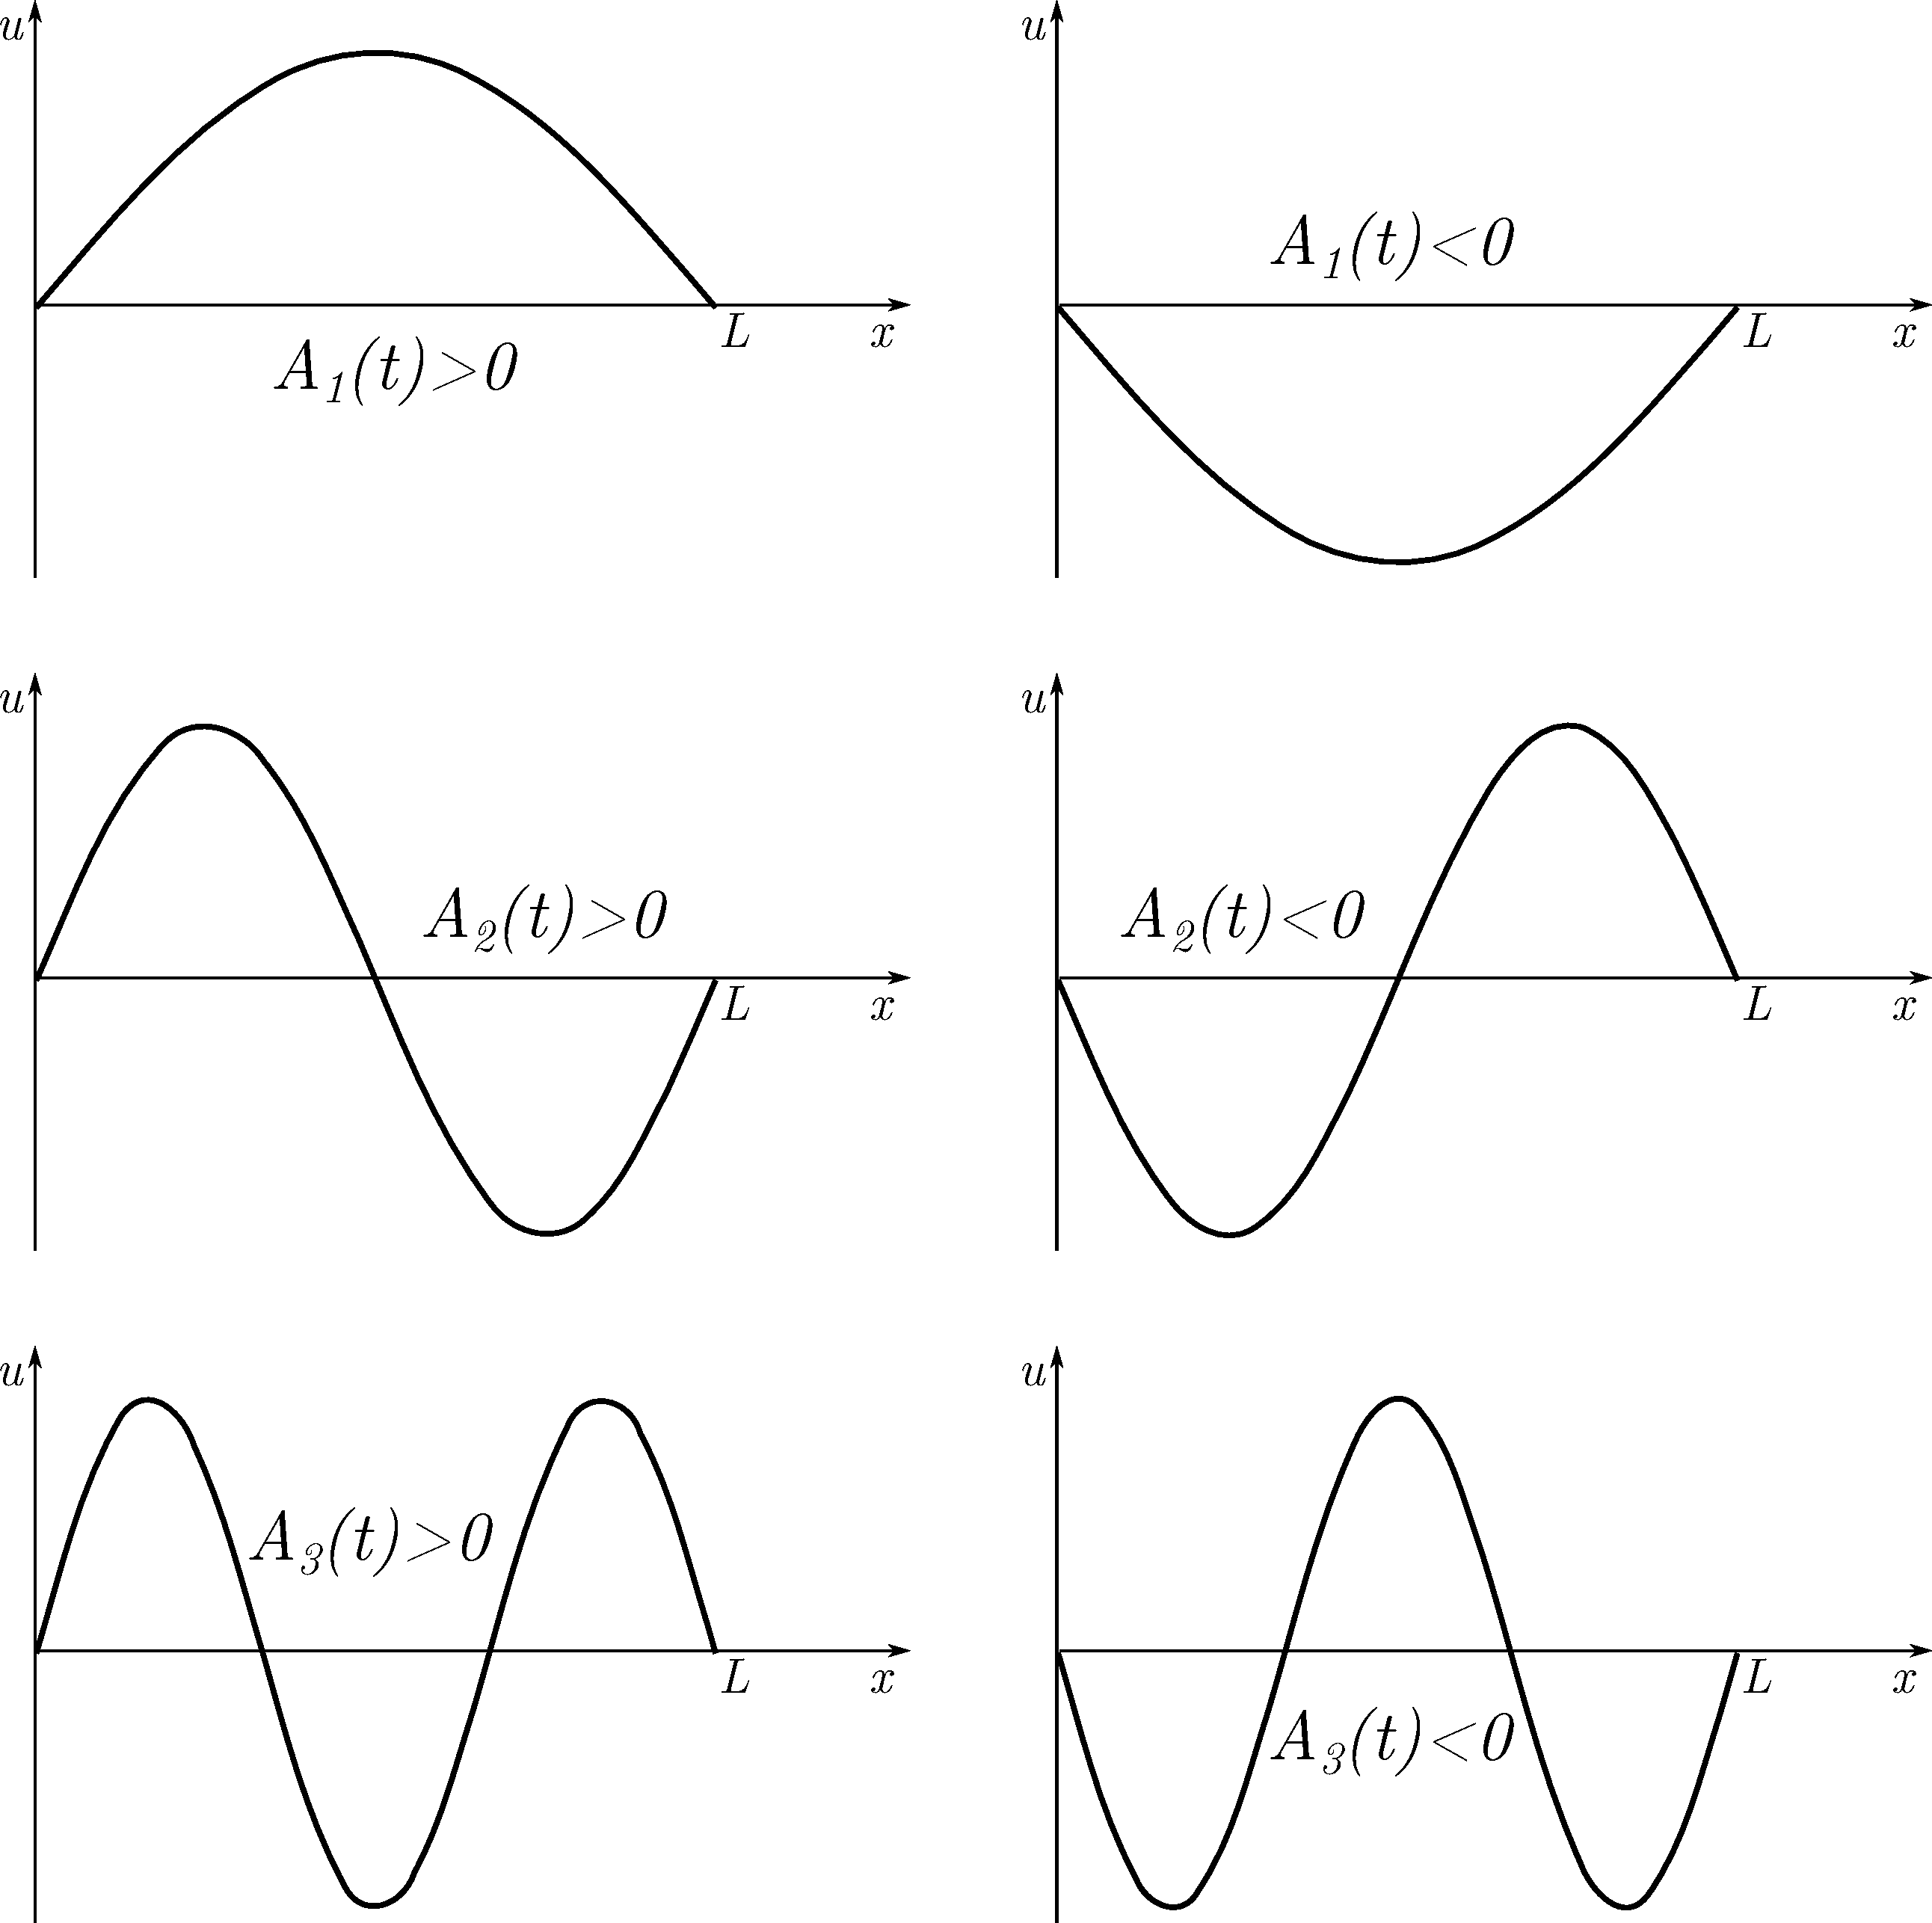
\includegraphics[width=\textwidth]{wave_modes.pdf}
	\caption{Alcune ``istantanee'' delle prime tre vibrazioni possibili a
$t$ fissato.}
	\label{wave_modes}
\end{figure}
\noindent
Come si pu\`o notare in fig. \ref{wave_modes}, dopo un tempo $T=\frac{2L}{c}$
si rivedono le stesse configurazioni: per $u_1$ \`e la priva volta, per $u_2$ la
seconda e per $u_3$ la terza volta che si osserva lo stesso grafico.\\
La sovrapposizione di vibrazioni con frequenza tutte multiple della stessa
frequenza di base
\[
	\frac{1}{T_1}= \frac{c}{2L}
\]
produce il suono armonioso della corda vibrante. La sovrapposizione
\[
	u= \sum_{m=1}^{\infty} u_m =
	\sum_{m=1}^{\infty} \left[ a_m \, cos \left( \frac{mc\pi}{L} t \right)
	+ b_m \, sin \left( \frac{mc\pi}{L} t \right) \right]
	 sin \left( \frac{m\pi}{L} x \right)
\]
\`e la soluzione completa.\\
Si definiscono quindi le condizioni iniziali
\[
	\begin{array}{l}
	u(0,x)= g(x)
 	\\
	u_t(0,x)= h(x)
	\end{array}
\]
Ponendo $t=0$ nell'espressione di $u$ e $u_t$
\[
	g(x)= \sum_{m=1}^{\infty} a_m \, sin \left( \frac{m\pi}{L} x \right)
\]
e
\[
	h(x)= \sum_{m=1}^{\infty} \frac{mc\pi}{L} b_m \, sin \left(
	\frac{m\pi}{L} x \right)
\]
Si sviluppano i dati $g(x)$ e $h(x)$ in serie di sole sinusoidi per $x \in
[0,L]$ effettuando il prolungamento continuo dispari all'intervallo $[-L,L]$.\\
I coefficienti sono quindi forniti da
\[
	a_m= \frac{2}{L} \int_0^L g(x) sin \left( \frac{m\pi}{L} x \right) dx
\]
\[
	b_m= \frac{2}{mc \pi} \int_0^L h(x) sin \left( \frac{m\pi}{L} x \right)
dx
\]
La funzione $u(t,x)$ cos\`i trovata risolve il problema almeno nel senso delle
distribuzioni.
Affinch\'e sia una soluzione in senso usuale occorre che si possa derivare due
volte in $dt$ ed in $dx$ sotto il segno di serie.
Questo \`e possibile se se i coefficienti $a_m$ e $b_m$ decadono almeno come
$\/m^4$: derivando due volte si producono addendi con coefficienti $m^a_m$,
$m^2b_m$. La condizione
\[
	m^2|a_m|\leq \frac{cost.}{m^2}, \;\;\; m^2|b_m|\leq \frac{cost.}{m^2}
\]
\`e sufficiente per garantire poi la convergenza dominata della serie ottenuta
derivando termine a termine.\\
La regolarit\`a $C^4$ per $g$ e $C^3$ per $h$ ($b_m$ ha gi\`a un $m$ a
denominatore) \`e una ipotesi sufficiente.\\
Osserviamo una diversit\`a fondamentale con l'equazione della diffusione. Per
questa ultima, qualunque sia la regolarit\`a del dato iniziale, i coefficienti
di Fourier della soluzione per $t>0$ decadono come $e^{-m^2 \pi^2 Dt/L}$ cio\`e
come $e^{-\alpha m^2}$ per $m \to +\infty$.
La soluzione ha in quel caso tutte le derivate in $dt$ e in $dx$ per $t>0$.
\`E questo l'effetto regolarizzante della diffusione, assente per l'equazione
della corda vibrante. Ora la soluzione \`e $C^k$ se i dati sono $g \in C^{k+2}$
e $h \in C^{k+1}$, $k\geq 2$. La regolarit\`a dei dati fornisce la regolarit\`a
della soluzione.\\
Non abbiamo ora soluzioni stazionare n\'e regime transitorio. In assenza di
attrito, la corda vibra all'infinito con una sovrapposizione di vibrazioni
periodiche stabilite dai dati iniziali.
\subsection{Dipendenza continua dai dati}
Indichiamo con $||u(t, \cdot)||_2$ la norma in $L^2$ della soluzione al tempo
$t$ fissato
\[
	||u(t, \cdot)||_2=
	\left(
	\int_0^L |u(t,x)|^2 dx
	\right)^{1/2}
\]
Per Parseval, dallo sviluppo di Fourier
\[
	u(t,x)= \sum_{m=1}^{\infty} \left[ a_m \, cos \left( \frac{mc\pi}{L} t
\right)
	+ b_m \, sin \left( \frac{mc\pi}{L} t \right) \right]
	 sin \left( \frac{m\pi}{L} x \right)
\]
segue
\[
	||u(t, \cdot)||_2^2 = \sum_{m=1}^{\infty} \left[ a_m \, cos \left(
	\frac{mc\pi}{L} t \right)
	+ b_m \, sin \left( \frac{mc\pi}{L} t \right) \right]^2
\]
usando $|cos \alpha |\leq 1$, $|sin \alpha |\leq 1$, $2ab \leq a^2 + b^2$
\[
	=\sum_{m=1}^{\infty} \left[ a_m \,
	+ b_m \, \right]^2 =
	\sum_{m=1}^{\infty} \left[ a_m^2 + b_m^2 + 2ab \right]
	\leq 2 \sum_{m=1}^{\infty} \left[ a_m^2 + b_m^2 \right]
\]
Sempre per Parseval
\[
	\sum_{m=1}^{\infty} a_m^2 =
	\int_0^L |g(x)|^2 dx = ||g||_2^2
\]
In quanto gli $a_m$ sono esattamente i coefficienti di Fourier di $g(x)$. I
$b_m$ sono i coefficienti di $h(x)$ divisi per $\frac{mc \pi}{L}\leq
\frac{c \pi}{L}$, quindi
\[
	\sum_{m=1}^{\infty} b_m^2 \leq \frac{L^2}{c^2 \pi^2}||h||^2_2
\]
Riassumendo
\[
	||u(t,\cdot)||_2^2 \leq M(||g||_2^2 + ||h||_2^2)
\]
Per linearit\`a, se $u_1$ e $u_2$ sono soluzioni del problema con dati di
Cauchy ($g_1,h_1$) e ($g_2,h_2$) rispettivamente, allora
\[
	||u_1(t,\cdot) - u_2(t,\cdot)||_2^2 \leq M(||g_1 - g_2||_2^2 + ||h_1 -
	h_2||_2^2)
\]
che esprime la dipendenza continua dai dati nel problema di Cauchy-Dirichlet
con dati di Dirichlet nulli.
\section{Il problema di Cauchy globale}
\subsection{Formula di D'Alambert}
Consideriamo il problema di Cauchy globale (L=$\infty$)
\[
	\begin{cases}
		u_{tt} - c^2 u_{xx}= 0 , \;\;\;\; t>0, \;\; x \in \mathbb{R} \\
		u(0,x)= g(x)\\
		u_t (0,x)= h(x)
	\end{cases}
\]
L'equazione
\[
	\left( \partial_t^2 -c^2 \partial_x^2 \right) u=0
\]
si scrive
\[
	\left( \partial_t -c \partial_x \right)\left( \partial_t + c
	\partial_x \right) u=0
\]
Posto
\[
	u(t,x)= v(y,\eta)
\]
con
\[
	y=x -ct, \;\;\; \eta= c+ ct
\]
si ha
\[
	\partial_tu= -c \partial_y v + c\partial_\eta v
\]
\[
	\partial_xu= \partial_y v + \partial_\eta v
\]
cio\`e
\[
	\partial_t - c \partial_x = -2c \partial_y
\]
\[
	\partial_t + c\partial_x = 2c \partial_n
\]
Abbiamo
\[
	u_{tt}- c^2u_{xx}= \underbrace{\left( \partial_t -c \partial_x
	\right)}_{-2c \partial_y}
	\underbrace{\left( \partial_t + c
	\partial_x \right)}_{2c \partial_\eta} u= -4c \, \partial_{y}
	\partial_{\eta} v=0
	\follows v_{yn}=0
\]
e l'equazione $v_{yn}=0$ ha per integrale generale
\[
	\frac{\partial}{\partial \eta} \left(
	\frac{\partial}{\partial y} v \right)=0
\]
\[
	\frac{\partial}{\partial \eta} v (y, \eta)=0
\]
\[
	v(y, \eta)= \int f(\eta) d\eta + \underbrace{ G(y) }_{\mathclap{
	\text{Costante rispetto a }\eta}}
\]
\[
	v(y, \eta)= F(\eta)+ G(y)
\]
con $F$, $G$ arbitrarie funzioni derivabili.\\
Tornando alle variabili iniziali
\[
	u(t,x)=F(x+ct)+G(x-ct)
\]
cio\`e $u$ \`e la sovrapposizione di due onde viaggianti (solitoni) in
direzioni opposte, alla medesima velocit\`a $c$.
\begin{figure}[H]
	\centering
	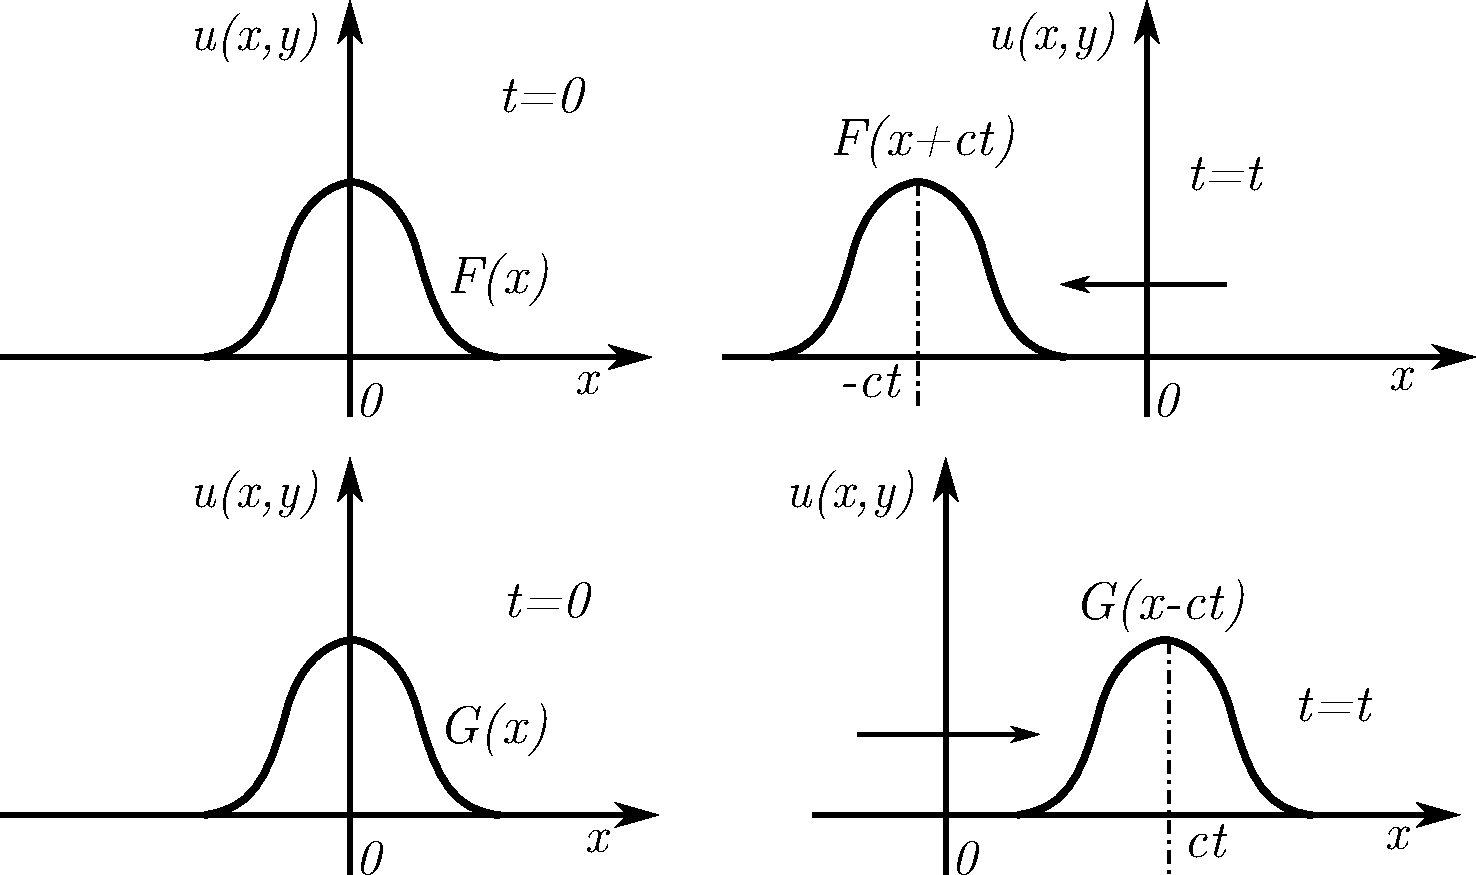
\includegraphics[width=\textwidth]{soliton.pdf}
	\caption{Onde viaggianti (solitoni).}
	\label{soliton}
\end{figure}
\noindent
Imponendo le condizioni iniziali
\[
	g(x)= u(0,x)= F(x)+ G(x)
\]
\[
	h(x)=u_t(0,x)=cF'(x)- cG'(x)
\]
(si \`e usato $u_t(t,x)= cF'(x+ct)- cG'(x+ct)$)
si ottiene
\[
	\left\{
	\begin{array}{ll}
		F+G= g\\
		cF-cG= H & H(x)= \int h(x)dx
	\end{array}
	\right.
\]
moltiplico la prima per $c$ e poi sommo o sottraggo; se sottraggo
\[
	2cG= cg - H
\]
se sommo
\[
	2cF= cg + H
\]
da cui
\[
	F=\frac{1}{2}g + \frac{1}{2c}H, \;\;\; G=\frac{1}{2}g-\frac{1}{2c}H
\]
ed infine
\[
	u(t,x)= \frac{1}{2}g(x+ct)+ \frac{1}{2}g(x-ct)+\frac{1}{2c}
	[H(x+ct)-H(x-ct)]
\]
\[
	= \frac{1}{2}g(x+ct)+ \frac{1}{2}g(x-ct)+\frac{1}{2c}
	\int_{x-ct}^{x+ct} h(y)dy
\]
Questa \`e nota come la formula di D'Alambert.\\
Definisce una soluzione di classe $C^2$ non appena $g \in C^2$ e $h \in C^1$.
Per come \`e stata ottenuta \`e l'unica soluzione di classe $C^2$ sotto tali
ipotesi di regolarit\`a dei dati.\\
Il metodo con cui \`e stata ottenuta mostra anche che $u$ \`e l'unica soluzione
di classe $C^k$ per dati $g \in C^k$, $h \in C^{k-1}$. Si noti l'assenza di
effetti regolarizzanti, la regolarit\`a dei dati stabilisce la regolarit\`a
della soluzione.\\
Dalla formula di D'Alambert si ottiene direttamente la dipendenza continua dai
dati secondo la norma di $L^{\infty}$
\[
	||f||_{\infty}= \sup_x|f(x)|
\]
Infatti
\[
	|u(t,x)| \leq \frac{1}{2}|g(x+ct)| + \frac{1}{2}|g(x-ct)|+
	\frac{1}{2c}\int_{x-ct}^{x+ct} |h(y)| dy
\]
\[
	\leq \frac{1}{2}||g||_\infty + \frac{1}{2}||g||_\infty+
	\frac{1}{2c}\int_{x-ct}^{x+ct} ||h||_\infty dy
\]
\[
	= ||g||_\infty + \frac{2ct}{2c}||h||_\infty= ||g||_\infty +
	t ||h||_\infty
\]
da cui
\[
	||u(t, \cdot)||_\infty \leq ||g||_\infty + t||h||_\infty
\]
Se ora $u_1$, $u_2$ sono soluzioni con rispettivi dati iniziali $(g_1,h_1)$ e
$(g_2,h_2)$, per linearit\`a abbiamo la stima di dipendenza continua dai dati.
\[
	||u_1(t, \cdot) - u_2(t, \cdot)||_\infty
	\leq ||g_1 -g_2||_\infty + t||h_1-h_2||_\infty
\]
Una ulteriore utile osservazione sulla formula di D'Alambert \`e che basta
saper risolvere il problema con $g=0$ ed $h$ arbitrario. Infatti la derivata in
$dt$ del termine corrispondente al dato $h$ vale
\[
	\frac{1}{2c}\partial_t \int_{x-ct}^{x+ct} h(y)dy=
	\frac{1}{2c}= [h(x+ct)c - h(x-ct)(-c)]=
\]
\[
	=\frac{1}{2} [h(x+ct) + h(x-ct)]
\]
che ha lo stesso aspetto del termine corrispondente al dato $g$. La formula di
D'Alambert diventa
\[
	u(t,x)= \frac{\partial}{\partial t}v_g(t,x)+ v_h(t,x)
\]
dove $v_H$ indica la soluzione del problema
\[
	\begin{cases}
		v_{tt}= c^2 v_{xx}\\
		v(0,x)= 0 \\
		v_t(0,x)= H(x)
	\end{cases}
\]
\subsection{Caratteristiche, Domini di dipendenza, Domini d influenza}
Nella rappresentazione
\[
	u(t,x)=F(x+ct) + G(x-ct)
\]
abbiamo il termine $F(x-ct)$ che \`e costante lungo la retta $\gamma^+$ di
equazione
\[
	x+ct=z, \;\;\; \text{$z$ fissato sull'asse $x$}
\]
nel piano $(x,t)$. Analogamente $G(x-ct)$ \`e costante lungo la retta
$\gamma^-$ di equazione
\[
	x-ct=z, \;\;\; \text{$z$ fissato sull'asse $x$}
\]
\begin{figure}[H]
	\centering
	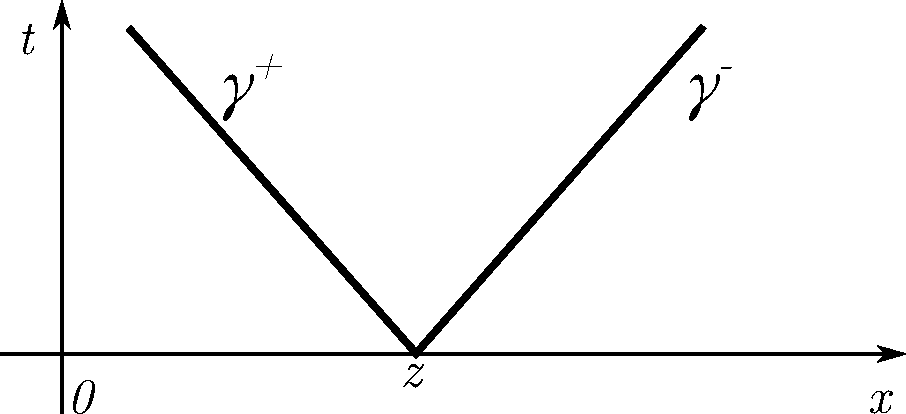
\includegraphics[width=0.6\textwidth]{char_rect.pdf}
	\caption{Rette caratteristiche.}
	\label{char_rect}
\end{figure}
\noindent
Queste rette che trasportano i dati iniziali si chiamano caratteristiche. Il
cono nel piano $(x,t)$ delimitato dalle caratteristiche per $(z,0)$ si chiama
dominio di influenza del punto $z$.
\begin{figure}[H]
	\centering
	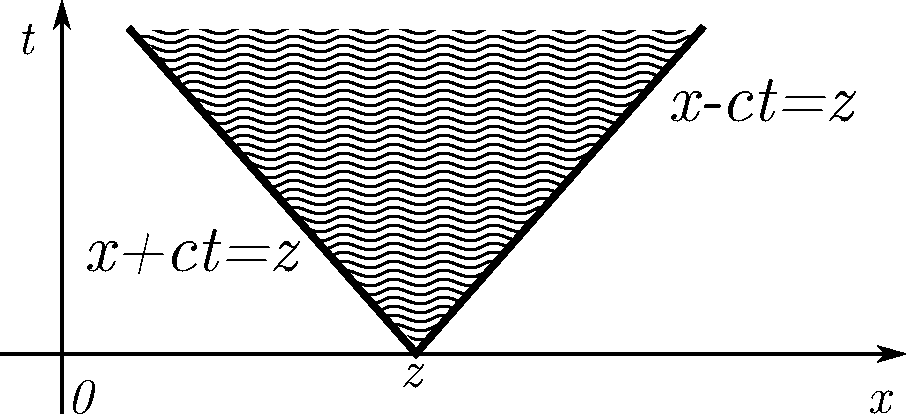
\includegraphics[width=0.6\textwidth]{infl_dom.pdf}
	\caption{Dominio di influenza.}
	\label{infl_dom}
\end{figure}
\noindent
I valori dei dati iniziali in $z$ influenzano i valori di $u(t,x)$ nei punti
del dominio cos\`i identificato. Una perturbazione iniziale localizzata in $z$
al tempo $t=0$, raggiunge il punto $x$ in un tempo
\[
	t=\frac{|x-z|}{c}
\]
In maniera simmetrica, la formula di D'Alambert dice che in un punto fissato
$(\bar{t}, \bar{x})$ il valore $u(\bar{t}, \bar{x})$ dipende solo dai valori
del dato iniziale $g(x)=u(0,x)$ nei due punti $\bar{x}+ c\bar{t}$ ed $\bar{x}-
c\bar{t}$ e dai valori del dato $h(x)=u_t(0,x)$ nell'intervallo $[\bar{x}-
c\bar{t}, \bar{x}+ c\bar{t}]$. Il valore $u(\bar{t}, \bar{x})$ dipende solo dai
valori di $g$, $h$ in $[\bar{x}- c\bar{t}, \bar{x}+ c\bar{t}]$.
Questo intervallo si chiama dominio di dipendenza e si ottiene tracciando le
caratteristiche per $(\bar{t}, \bar{x})$ fino ad incontrare l'asse $x$ nei
punti $\bar{x} - c\bar{t}$, $\bar{x}+ c\bar{t}$
\begin{figure}[H]
	\centering
	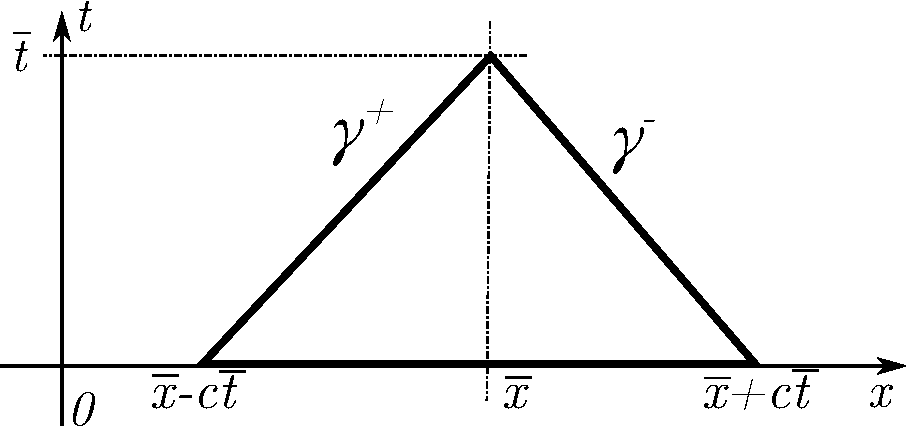
\includegraphics[width=0.6\textwidth]{dep_dom.pdf}
	\caption{Dominio di dipendenza.}
	\label{dep_dom}
\end{figure}
\noindent
Sempre da
\[
	u(t,x)= F(x+ct) + G(x-ct)
\]
si ottiene un'altra interessante propriet\`a.\\
Il rettangolo in fig. \ref{char_recta} si chiama rettangolo caratteristico.
\vspace{5mm}
\begin{figure}[H]
	\centering
	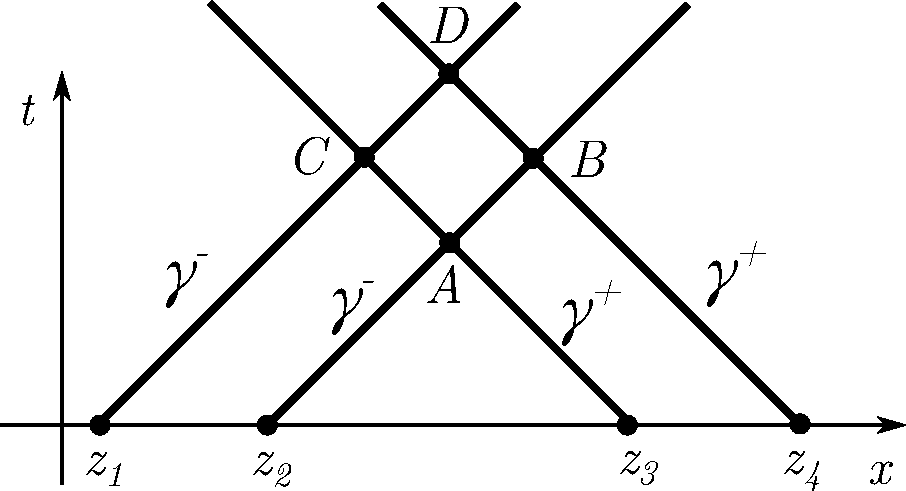
\includegraphics[width=0.6\textwidth]{char_recta.pdf}
	\caption{Rettangolo caratteristico.}
	\label{char_recta}
\end{figure}
\noindent
Abbiamo
\[
	\begin{array}{lcl}
		F(A)=F(C) 	&,&	F(D)=F(B)\\
		G(A)=G(B)	&,&	G(C)=G(D)
	\end{array}
\]
da cui
\[
	u(A)+u(D)=F(A)+F(G)+F(D)+G(D)
\]
coincide con
\[
	u(B)+u(C)= F(B)+G(B)+F(C)+G(C)
\]
Da
\[
	u(A)+u(D)=u(C)+u(B)
\]
segue che nota $u$ in tre vertici si trova $u$ nel quarto vertice.

\subsection{Conservazione dell'energia}
Si ricorda che l'energia \`e data da
\[
	E(t)=\frac{1}{2} \intR \left(
	\rho_0 u_t^2 + \tau u_x^2
	\right) dx
\]
Il teorema di Parseval afferma
\[
	\intR |f(x)|^2 dx =
	\frac{1}{2\pi}
	\intR |\hat{f}(\lambda)|^2d \lambda
\]
Perci\`o, dato $f=u_t \follows |\hat{f}|^2=|v_t|^2$ e
$f=u_x \follows |\hat{f}|^2=|i\lambda v|^2=\lambda^2|v|^2$
\[
	E(t)= \frac{1}{4 \pi} \intR
	\left(
	\rho_0 |v_t|^2 + \tau \lambda^2 |v|^2
	\right) d\lambda
\]
La derivata di $|g(t)|^2$ con $g(t)$ a valori complessi pu\`o essere ottenuta
considerando
\[
	|g(t)|^2= g(t)\underbracket{g^*(t)}_{\mathclap{\text{Coniugato}}}
\]
\[
	\frac{d}{dt}|g(t)|^2=
	g'(t) g^{*} (t) + g(t)(g^{*})'(t)= g'(t)g^{*}(t)+
	\left(
	g'(t)g^*(t)
	\right)^*
\]
\[
	=2 {\mathcal Re} \left\{ g'(t)g^*(t) \right\}
	=2 {\mathcal Re} \left\{ (g'(t)g^*(t))^* \right\}
	=2 {\mathcal Re} \left\{ (g'(t))^* g(t) \right\}
\]
Ora
\[
	E'(t)= \frac{1}{4\pi} \intR \left[
	\rho_0 \, 2 {\mathcal Re} \{v_t^* \, v_{tt}\}+
	\tau \lambda^2 \, 2 {\mathcal Re} \{ v \,v_t^* \}
	\right] d \lambda
\]
\[
	=\frac{1}{2\pi} \intR \left[
	{\mathcal Re} \{ \rho_0 v_t^* v_{tt} + \tau \lambda^2 vv_t^* \}
	\right] d \lambda
\]
\[
	=\frac{1}{2\pi} \intR \left[
	{\mathcal Re} \{ v_t^* (\rho_0 v_{tt} + \tau \lambda^2 v) \}
	\right] d \lambda
\]
Data $\rho_0 v_{tt} + \tau \lambda^2 v=0$ dalla trasformata di $\rho_0 u_{tt} -
\tau u_{xx}= 0$
\[
	=\frac{1}{2\pi} \intR \left[
	{\mathcal Re} \{ v_t^* \, 0 \}
	\right] d \lambda = 0
\]

Si ottiene $E'(t)=0$, perci\`o l'energia non varia nel tempo e quindi si
conserva $\follows E(t)=E(0)$.\\
Di conseguenza
\[
	\intR (\rho_0 u_t^2 + \tau u_x^2)dx=
	\intR (\rho_0h^2 + \tau (g')^2)dx
\]
Si consideri ora la soluzione $u=(u_1 - u_2)$, si ottiene
\[
	\intR \left[
	\rho_0 (u_1 - u_2)_t^2 + \tau (u_1 - u_2)_x^2
	\right]dx=
	\intR \left[
	\rho_0 (h_1 - h_2)_t^2 + \tau (g_1' - g_2')_x^2
	\right]dx
\]
che mostra l'unicit\`a e la dipendenza continua dai dati.

\subsection{Soluzioni attraverso la trasformata di Fourier}
Presa la trasformata del problema globale
\[
	u_{tt} - c^2u_{xx}
	\substack{\displaystyle{\mathscr{F}} \\ \follows}
	v_{tt} + c^2 \lambda^2 v = 0
\]
la cui equazione caratteristica risulta
\[
	\xi^2 +c^2 \lambda=0 \follows \xi=\pm ic \lambda
\]
La soluzione perci\`o
\[
	v(t,\lambda)= a(\lambda)e^{ic\lambda t} + b(\lambda)e^{-ic\lambda t}
\]
\[
	a(\lambda)= {\mathscr{F} \left( A(x) \right)} \;\;\;
	b(\lambda)= {\mathscr{F} \left( B(x) \right)}
\]
mentre il prodotto per un fasore trasla di $ct$.
Quindi
\[
	u(t,x)= A(x+ct) + B(x-ct)
\]
abbiamo nuovamente la somma di due solitoni.\\
Si determinano $a(\lambda)$ e $b(\lambda)$, di conseguenza anche $A(x)$ e
$B(x)$, con le condizioni iniziali.
\[
	v(0,\lambda)=\hat{g}(\lambda)
\]
\[
	v_t(0,\lambda)=\hat{h}(\lambda)
\]
\[
	v_t(t,\lambda)= ic\lambda \left(
	a(\lambda)e^{ic\lambda t} - b(\lambda)e^{-ic\lambda t} \right)
\]
\[
	\left\{
	\begin{array}{lcl}
		a(\lambda)+b(\lambda)=\hat{g}(\lambda) \\
		ic\lambda (a(\lambda)-b(\lambda))= \hat{g}(\lambda)
		&\Rightarrow&
		\hat{g}(\lambda) = i\lambda (ca(\lambda) - cb(\lambda))
	\end{array}
	\right.
\]
Bisogna perci\`o procurarsi
\[
	H(x)= \int h(x)dx
\]
Considerato che, dato $H'=h$, si ha $\hat{h}=i\lambda \hat{H}$
\[
	\left\{
	\begin{array}{l}
		a(\lambda)+b(\lambda)=\hat{g}(\lambda) \\
		ca(\lambda)-cb(\lambda)= \hat{H}(\lambda)
	\end{array}
	\right.
\]
$A(x)$e $B(x)$ applicate le condizioni iniziali risultano
\[
	a(\lambda)=\frac{1}{2c}(c\hat{g}+ \hat{H})
	= \frac{1}{2}\hat{g}+ \frac{1}{2c}\hat{H}
\]
\[
	b(\lambda)=\frac{1}{2c}(c\hat{g}- \hat{H})
	= \frac{1}{2}\hat{g}- \frac{1}{2c}\hat{H}
\]
che antitrasformando
\[
	\left\{
	\begin{array}{l}
		A(x)=\frac{1}{2}g + \frac{1}{2c}H \\
		B(x)=\frac{1}{2}g - \frac{1}{2c}H
	\end{array}
	\right.
\]
dove
\[
	H(x)= \int h(c) dx
\]
in senso generalizzato.
\[
	u(t,x)= A(x +ct) + B(x-ct)=
	\frac{1}{2}[g(x+ct)+ g(x-ct)]+
	\frac{1}{2c}[H(x+ct)-H(x-ct)]
\]
rappresenta la formula di D'Alambert.\\
Nel caso singolare questa \`e l'ultimo step; Nel caso regolare, cio\`e con
funzioni regolari, si pu\`o anche scrivere
\[
	\frac{1}{2c}[H(x+ct)-H(x-ct)]=
	\frac{1}{2c}\int_{x-ct}^{x+ct} h(y)dy
\]
Si nota che se i dati hanno una singolarit\`a sul punto $z$ (discontinuit\`a
della funzione o di qualche derivata) allora la soluzione \`e singolare lungo
le caratteristiche
\[
	x \pm ct=z
\]
spiccate da $z$. Le singolarit\`a viaggiano lungo le caratteristiche a
velocit\`a $c$.\\
Tra tutte queste soluzioni, nel prossimo paragrafo si evidenza la soluzione
fondamentale.
\subsection{Soluzione fondamentale}
Si consideri il problema
\[
	\left\{
	\begin{array}{l}
		u_{tt}-c^2u_{xx}=0\\
		u(0,x)=0\\
		u_t(0,x)=\delta
	\end{array}
	\right.
\]
esso consiste nell'applicare un impulso unitario localizzato in $x=0$. \\
Poich\'e $H'=\delta$ \`e risolto dalla funzione di Heaviside (gradino unitario)
\[
	H(x)=1, \;\;\; x \in [0, \infty) \;\;\;\;\;
	H(x)=0, \;\;\; x \in (0,\infty)
\]
\begin{figure}[H]
	\centering
	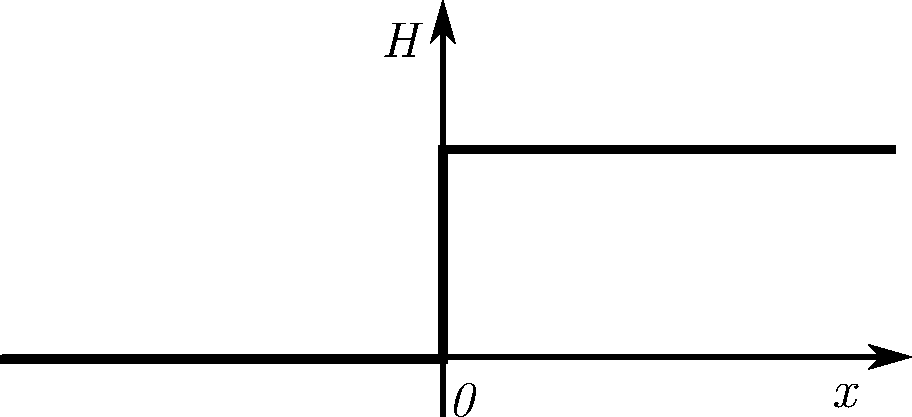
\includegraphics[width=0.6\textwidth]{heaviside.pdf}
	\caption{Funzione di Heaviside.}
	\label{heaviside2}
\end{figure}
\noindent
la soluzione fondamentale \`e
\[
	k(t,x)= \frac{1}{2c}(H(x+ct)- H(x-ct))
\]
Essa vale $1/(2c)$ nel dominio di influenza di vertice l'origine e $0$ altrove
\begin{figure}[H]
	\centering
	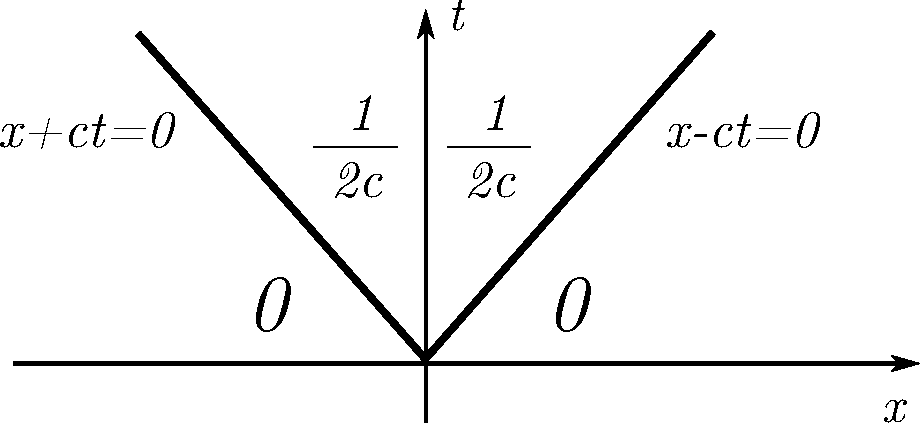
\includegraphics[width=0.6\textwidth]{fond_dom.pdf}
	\caption{Dominio di influenza per la soluzione fondamentale.}
	\label{fond_dom}
\end{figure}
\noindent
La singolarit\`a iniziale in  $x=0$ diventa una singolarit\`a di salto lungo la
caratteristica per l'origine.
Ad un tempo $t$ fissato, il grafico di $k(t,x)$
\begin{figure}[H]
	\centering
	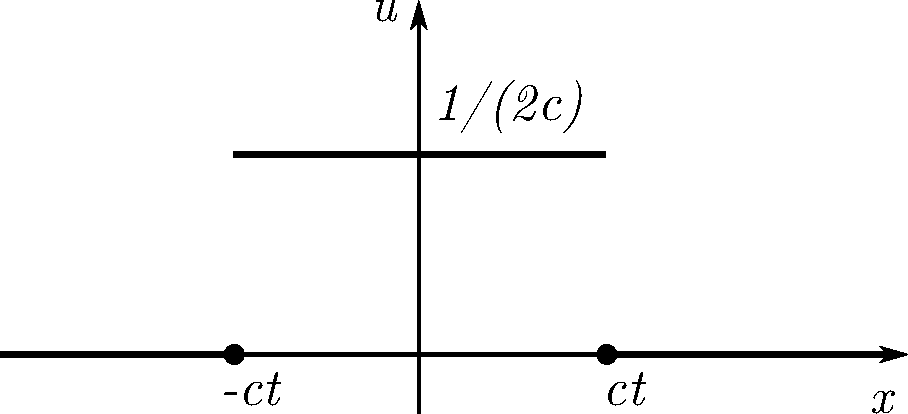
\includegraphics[width=0.6\textwidth]{fond_sol.pdf}
	\caption{Soluzione fondamentale.}
	\label{fond_sol}
\end{figure}
\noindent
Si noti che, fissare $u_t(0,x)=\delta(x)$ e $u(0,x)=0$,
significa anche a dire $u(t,0)= $ al gradino unitario in $x=0$, cio\`e
$u(t,0)=0$ con $t\leq 0$ e $u(t,0)=1/(2c)$ con $t>0$.\\
Abbiamo ottenuto la soluzione fondamentale dalla formula di D'Alambert.
Viceversa dalla espressione della soluzione fondamentale si pu\`o riottenere
tale formula.
Infatti, per traslazione, il problema
\[
	\left\{
	\begin{array}{l}
		u_{tt}-c^2u_{xx}=0\\
		u(0,x)=0\\
		u_t(0,x)=\delta_y
	\end{array}
	\right.
\]
\`e risolto da
\[
	k(t,x-y)= \frac{1}{2c}(H(x-y+ct)- H(x-y-ct)),
\]
funzione che vale $1/(2c)$ per $y-ct\leq x \leq y+ct$e che vale $0$ altrove.
La soluzione del problema generale
\[
	\left\{
	\begin{array}{l}
		u_{tt}-c^2u_{xx}=0\\
		u(0,x)=0\\
		u_t(0,x)=h(x)
	\end{array}
	\right.
\]
si ottiene per sovrapposizione tramite la convoluzione
\[
	u(t,x)= \intR k(t,x-y)h(y)dy
\]
Dunque
\[
	u(t,x)= \frac{1}{2c} \intR H(x-y+ct) h(y) dy -
	\frac{1}{2c} \intR H(x-y-ct) h(y) dy
\]
\[
	=\frac{1}{2c} \int_{-\infty}^{x+ct} h(y) dy -
	\frac{1}{2c} \int_{-\infty}^{x-ct} h(y) dy
	=\frac{1}{2c} \int_{x-ct}^{x+ct} h(y) dy
\]
che \`e la formula di D'Alambert per $u(0,x)=g(x)=0$. Abbiamo gi\`a visto che
la formula fondamentale si deduce da questo caso $g=0$.
